\hypertarget{_tutorial_scene_state___start_8cpp}{}\section{C\+:/\+H\+A\+L/\+P\+G関係/03\+\_\+作成プログラム/03\+\_\+\+H\+A\+L授業/就職作品/\+Project/source/02\+\_\+\+Scene/\+Scenes/\+Tutorial\+Scene/\+Tutorial\+Scene\+State/\+Tutorial\+Scene\+State\+\_\+\+Start/\+Tutorial\+Scene\+State\+\_\+\+Start.cpp ファイル}
\label{_tutorial_scene_state___start_8cpp}\index{C\+:/\+H\+A\+L/\+P\+G関係/03\+\_\+作成プログラム/03\+\_\+\+H\+A\+L授業/就職作品/\+Project/source/02\+\_\+\+Scene/\+Scenes/\+Tutorial\+Scene/\+Tutorial\+Scene\+State/\+Tutorial\+Scene\+State\+\_\+\+Start/\+Tutorial\+Scene\+State\+\_\+\+Start.\+cpp@{C\+:/\+H\+A\+L/\+P\+G関係/03\+\_\+作成プログラム/03\+\_\+\+H\+A\+L授業/就職作品/\+Project/source/02\+\_\+\+Scene/\+Scenes/\+Tutorial\+Scene/\+Tutorial\+Scene\+State/\+Tutorial\+Scene\+State\+\_\+\+Start/\+Tutorial\+Scene\+State\+\_\+\+Start.\+cpp}}


チュートリアルシーンステート(スタート)Class  


{\ttfamily \#include \char`\"{}Tutorial\+Scene\+State\+\_\+\+Start.\+h\char`\"{}}\newline
{\ttfamily \#include \char`\"{}../../\+Tutorial\+Scene.\+h\char`\"{}}\newline
{\ttfamily \#include \char`\"{}../\+Tutorial\+Scene\+State\+\_\+\+End/\+Tutorial\+Scene\+State\+\_\+\+End.\+h\char`\"{}}\newline
{\ttfamily \#include $<$Scene\+Manager\textbackslash{}\+Scene\+Manager.\+h$>$}\newline
{\ttfamily \#include $<$Resource\+Manager\textbackslash{}\+Resource\+Manager.\+h$>$}\newline
{\ttfamily \#include $<$Convert\+To\+Frame\textbackslash{}\+Meter\+To\+Frame\textbackslash{}\+Meter\+To\+Frame.\+h$>$}\newline
{\ttfamily \#include $<$Keyboard\textbackslash{}\+Keyboard.\+h$>$}\newline
{\ttfamily \#include $<$Game\+Object\+Manager/\+Game\+Object\+Manager.\+h$>$}\newline
{\ttfamily \#include $<$2\+D/\+U\+I/\+Tutorial\+Logo/\+Tutorial\+Logo\+Factory/\+Tutorial\+Logo\+Factory.\+h$>$}\newline
{\ttfamily \#include $<$2\+D/\+U\+I/\+Push\+Space\+Logo/\+Push\+Space\+Logo\+Factory/\+Push\+Space\+Logo\+Factory.\+h$>$}\newline
Tutorial\+Scene\+State\+\_\+\+Start.\+cpp の依存先関係図\+:
\nopagebreak
\begin{figure}[H]
\begin{center}
\leavevmode
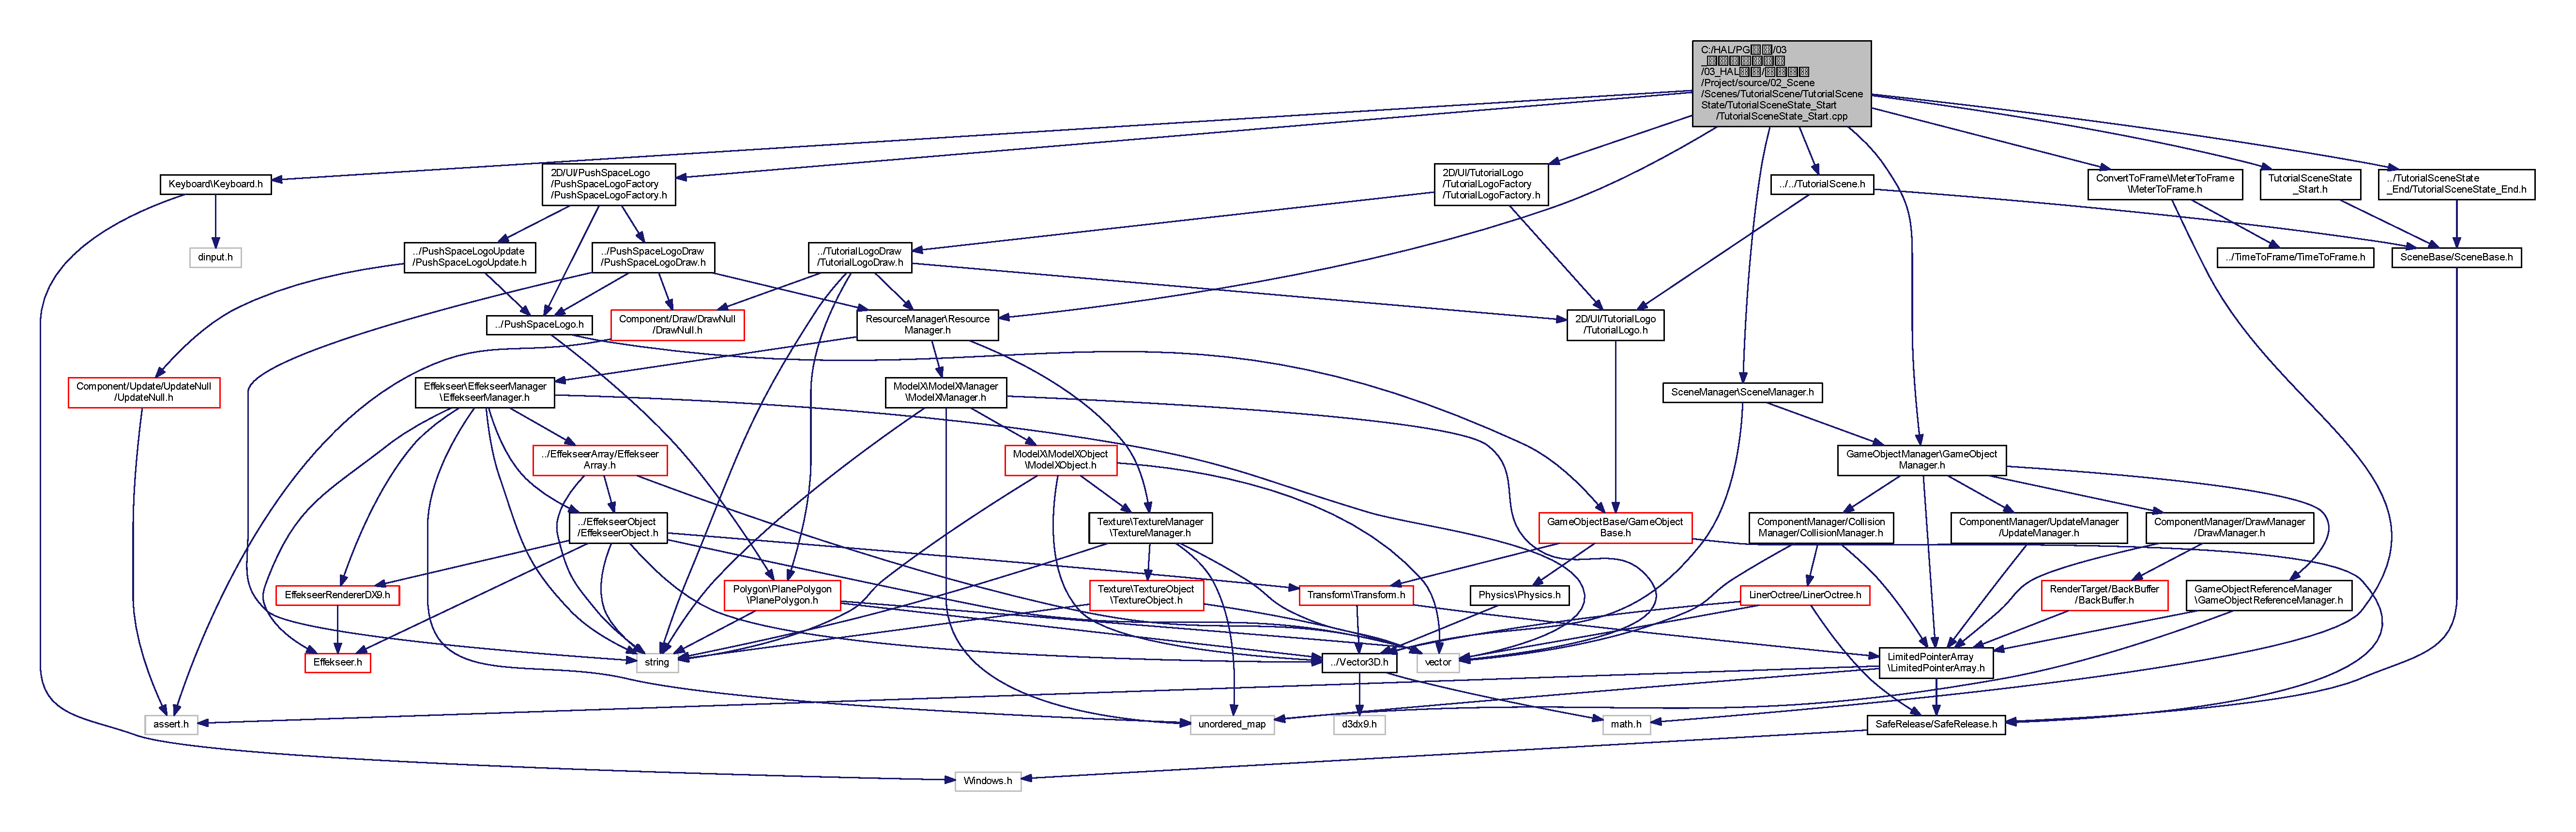
\includegraphics[width=350pt]{_tutorial_scene_state___start_8cpp__incl}
\end{center}
\end{figure}


\subsection{詳解}
チュートリアルシーンステート(スタート)Class 

\begin{DoxyAuthor}{著者}
Kai Araki 
\end{DoxyAuthor}
\begin{DoxyDate}{日付}
2018/07/24 
\end{DoxyDate}
